
\vspace{-1.0\baselineskip}
\section{Introduction}
\label{sec:intro}
\vspace{-0.3\baselineskip}

% depth normal is natural ability, without groud truth
Human beings are professional in recovering the 3D geometry of observed natural scenes at a very detailed level in real-time, even from a single image. 
More impressively, we leaned to achieve this ability only through visual perception of consecutive changing of outside world and ego-motion, \ie watching videos. 
Practically, being able to do reconstruction for unlabeled videos can be widely applied to large amount of real applications like augmented reality, robotics \etc

Therefore, letting computer manage dense 3D reconstruction ability by watching videos is a central problem of computer vision. 
One group of approaches is geometric based method depend on feature matching, \eg structure from motion (SFM) \cite{wu2011visualsfm} \etc, or color matching, \eg DTAM \cite{NewcombeLD11}, \etc  Since our world exists in 3D space and the images generated follows camera geometry, as long as the matching from corresponding frames are correct, we can exactly solve the 3D structure. 
However, theoretically, those methods does not explain why human can also do reconstruction from a single image by observing videos. In addition, they can easily fail once the feature matching is wrong, \eg when SIFT \cite{lowe2004distinctive}  feature meets a wall with white color. 
Thus, geometric based methods do not have the ability to discover new reconstruction cues from videos, and ignore the information inside monocular images.

\begin{figure}
\centering
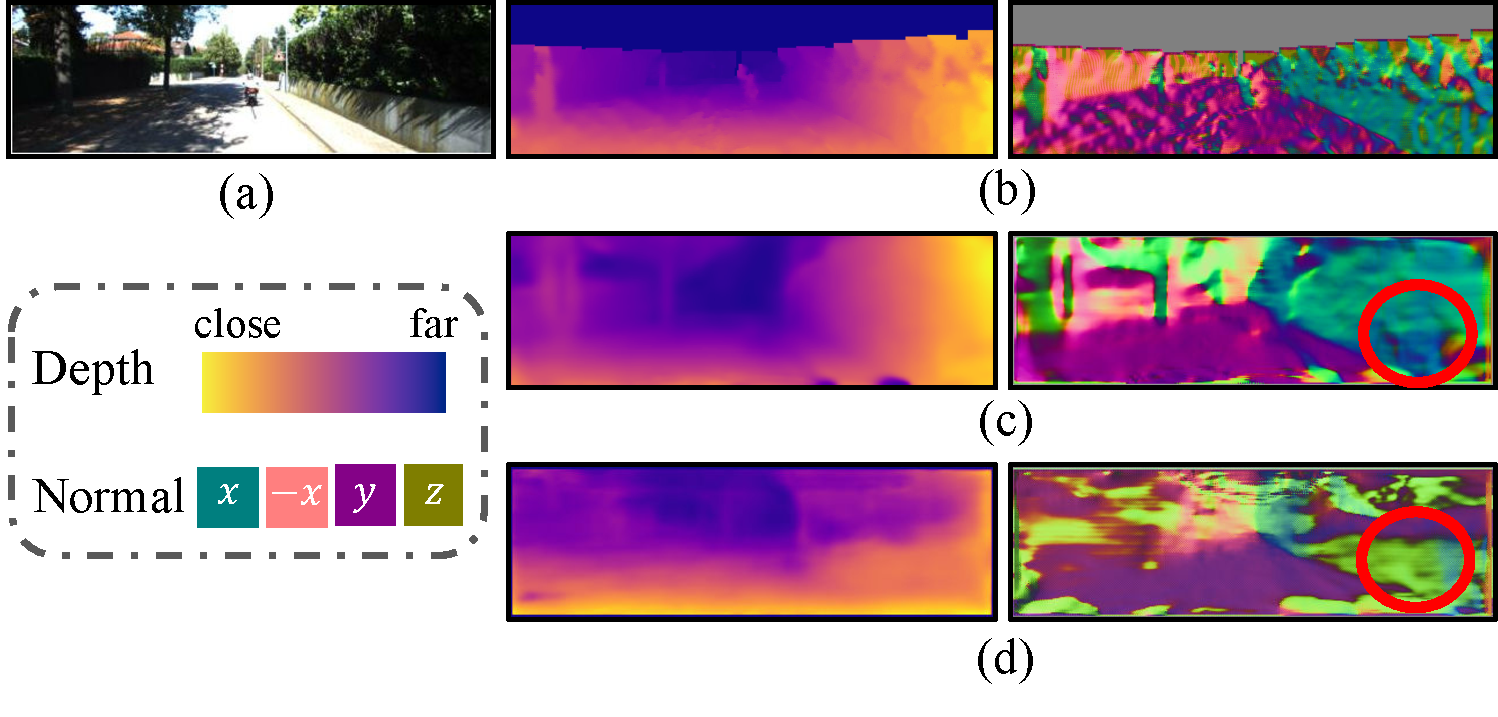
\includegraphics[width=0.45\textwidth]{figures/visual_comparison_comp.pdf}
\caption{Comparison of visual outputs of our model with and without depth-normal consistency. Top to bottom: (b) ground truth depth and normal, (c) our results with depth-normal consistency, (d) our results without depth-normal consistency. Note in the red circle region, our model with depth-normal consistency predicts both depth and normal correct, but the model without depth-normal consistency fails in normal estimation.}
\label{fig:visual_comparison}
\end{figure}

Another way to do 3D reconstruction is learning based method, where the reconstruction cues can be incrementally discovered and applied by keeping feeding in unobserved videos. Currently, with the development of pixel-wise prediction via deep learning such as fully convolutional network (FCN) \cite{long2015fully}, supervised learning of depth, \eg \cite{eigen2014depth,ummenhofer2016demon}, achieved impressive results over public datasets like KITTI \cite{geiger2012we}, NYUv2 \cite{silberman2012indoor} and SUN3D \cite{xiao2013sun3d}. 
Nevertheless, collecting ground truth depth is almost impossible for most online videos, where the learned models are hard to generalize. 
Thus, learning depth with unlabeled videos attracts lots of attention currently. Most recently,
\cite{zhou2017unsupervised} propose to learn a depth FCN for a single image from videos. The idea is for training, rather than using ground truth depth, they warp the target image to other consecutive video frames based on the predicted depths and relative motions, and match the photometry between the warped frames and observed frames (detailed in \secref{sec:preliminaries}). Then, the matching errors are back-propagated to the network, which supervise the prediction of depths. Similar idea was applied in depth prediction when stereo pairs is available~\cite{GargBR16,godard2016unsupervised}.
%\cite{godard2016unsupervised} apply FCN to predict depth from a single image,  photometric matching from stereo pairs, and back-propagate the matching error to the network. Later works \cite{zhou2017unsupervised,Vijayanarasimhan17} extends to using information from consecutive video frames by introducing camera ego-motion. 
Although those methods are able to do single image depth estimation, the results are still far from satisfactory. As shown at \figref{fig:visual_comparison}(d), the depth results from \cite{zhou2017unsupervised} does not well represent the structure of given scene, especially when visualized with computed normals. 
This is mostly due to photometric matching is ambiguous, \ie a color in source frames can be matched to multiple similar colors in target frames. Although researchers usually apply smoothness of depths \cite{zhou2017unsupervised} to reduce the ambiguity, it is often a weak constraint over neighboring pixels, yielding non-satisfied normal results.

\begin{figure*}[t]
\centering
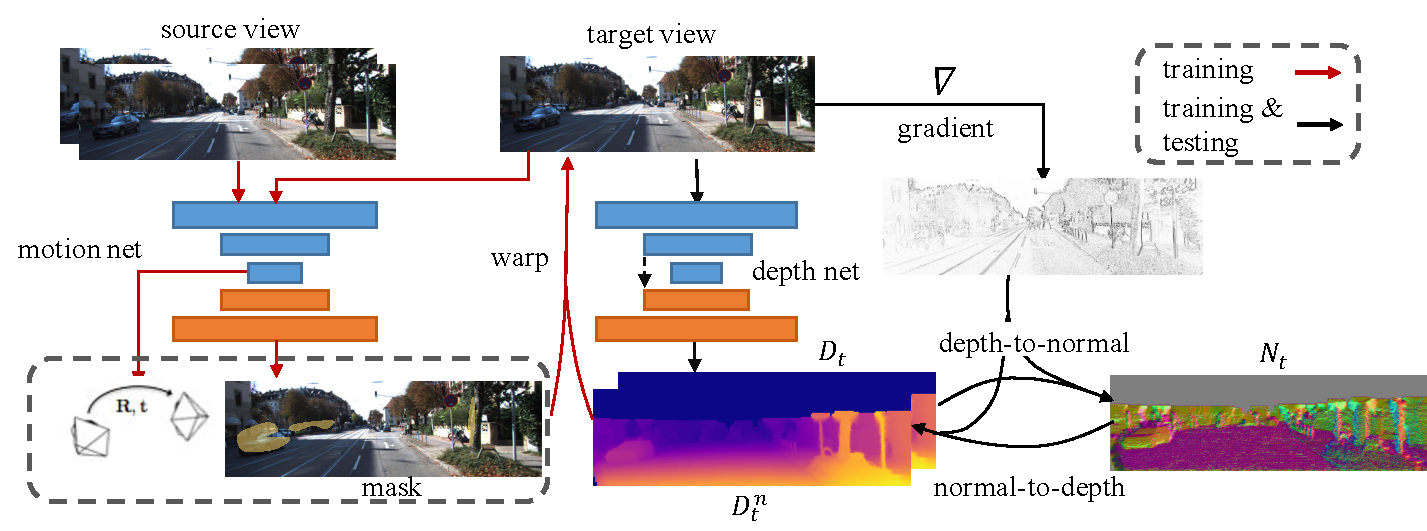
\includegraphics[width=0.85\textwidth]{figures/pipeline_comp.pdf}
\caption{Framework of our approach (Details at \secref{sub:framework}).}
\label{fig:pipeline}
\vspace{-1.3\baselineskip}
\end{figure*}

Our work falls in the scope of learning based 3D reconstruction with videos following the work of \cite{zhou2017unsupervised}, but is a step further towards learning a regularized 3D geometry with particular awareness of normal representation. 
We are motivated by the fact that human beings are able to explicitly point out the normal direction of each pixel in an image. Actually, we are more sensitive to normal than depth, \eg one could precisely point out the normal direction of a pixel while could only roughly know the exact depth. 
Thus, we induce normal representation in the pipeline and developed an edge-aware depth-normal consistency constrain inside the network which better regularizes the learning of depths (\secref{sec:approach}). 
There are several advantages of having normal estimated. For instance, it gives explicit understanding of normal for learned models.  In addition, it provides higher order interaction between estimated depths, which is beyond local neighbor relationships. Last, additional operations, \eg Manhattan assumption, over normals could be further integrated.
%Last but not the least, additional relationship, such as Manhattan world \cite{}, could be easily integrated with nor.
As shown at \figref{fig:visual_comparison}(c), with the help such a constrain, our recovered geometry is comparably better. We did extensive experiments over the publish KITTI and NYUv2 dataset, and show our algorithm can achieve relative 20$\%$ improvement over the state-of-the-art method on depth estimation and 10$\%$ improvement on predicted normals. More importantly, the training converges around 3$\times$ faster. These demonstrate the efficiency and effectiveness of our approach.
% recent work stereo, (eccv 2016, cvpr 2017), motion (cvpr 2017)
% matching can be easy, keep local structure for regularize depth is important,  

% normal is the most important structure that can explicit represent, no work on this

% we focus on 1: regularize depth, 2: explicit represent normal, 3: enforce the consistency


\vspace{-0.6\baselineskip}
\subsection{Framework}
\label{sub:framework}
\vspace{-0.3\baselineskip}

\figref{fig:pipeline} illustrate an overview of our approach. For training, we apply supervision from view synthesis following \cite{zhou2017unsupervised}. Specifically, the depth network (middle) takes only the target view as input, and
outputs a per-pixel depth map $D_t$, based on which a normal map $N_t$ is generated by the depth-to-normal layer. Then, given the $D_t$ and $N_t$, a new depth map $D_t^n$ is estimated from the normal-to-depth layer using local orthogonal compatibility between depth and normals. Both of the layers takes in image gradient to avoid non-compatible pixels involving in depth and normal conversion (detailed in \secref{sec:approach}).
Then, the new depth map $D_t^n$, combined with poses and mask predicted from the pose network (left), are then used to inversely warp the source views to reconstruct the target view, and errors are back propagated through both networks. Here the normal representation naturally serves as a regularization for depth estimation. Finally, for training loss, additional to the usually used photometric reconstruction loss, we also add in smoothness over normals, which induces higher order interaction between pixels (\secref{sub:training_losses})

After the model is trained, given a new image,  we first infer per-pixel depth value and then compute the normal value, yielding consistent prediction between the two predictions.
% problem normal can be locally estimated , while depth need global.  Another brach purely for normal


% In summary, the contributions of this paper lie in three folds:
% \begin{enumerate}
%     \item We provide to explicitly represent normal from images via unsupervised depth estimation, which is useful in real applications and serves as a regularization for depth prediction.
%     \item We

% \end{enumerate}

